\documentclass[tikz]{standalone}
\usepackage{pgfplots}
\pgfplotsset{compat=1.15}
\usepackage{mathrsfs}
\usetikzlibrary{arrows,calc}
\usepackage{tkz-euclide}
\pagestyle{empty}
\usepackage{fp}

\definecolor{AngleClr}{rgb}{0,0.39215686274509803,0}
\definecolor{ShapeClr}{rgb}{0.6,0.2,0}

\begin{document}

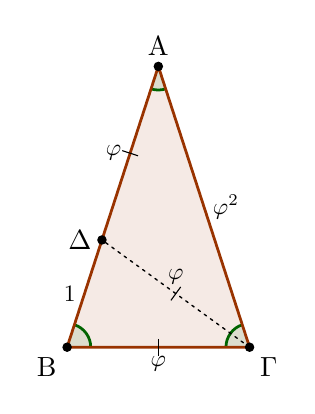
\begin{tikzpicture}[scale=.75]
\tkzSetUpLine[line width=1pt,color=black]
\tkzSetUpPoint[fill=black]

\def\LL{5}
\FPeval{\Xx}{0.3090 * \LL}
\FPeval{\Yy}{0.9510 * \LL}
\FPeval{\R}{2*\Xx}
\tkzDefPoints{-\Xx/0/B,0/\Yy/A,\Xx/0/C}

\tkzInterLC(A,B)(C,B) \tkzGetFirstPoint{D}

\tkzFillPolygon[fill=ShapeClr,fill opacity=0.1](A,B,C)
\tkzFillAngles[fill=AngleClr,size=.4,fill opacity=0.1](C,B,A A,C,B B,A,C)
\tkzMarkAngles[line width=1pt,size=.4,color=AngleClr](C,B,A A,C,B B,A,C)

\tkzDrawPolygon[color=ShapeClr](A,B,C)
\tkzDrawPoints[size=3](A,B,C,D)
\tkzLabelPoint[above](A){$\rm A$}
\tkzLabelPoint[below left](B){$\rm B$}
\tkzLabelPoint[below right](C){$\rm \Gamma$};
\tkzLabelPoint[left](D){$\rm \Delta$};

\tkzDrawSegment[line width=0.5pt,color=black,dashed,dash pattern=on 1pt off 1.75pt](C,D)

\tkzMarkSegments[mark=|,size=3](B,C C,D D,A)


\tkzLabelSegment[scale=0.85,below](B,C){$\varphi$}
\tkzLabelSegment[scale=0.85,above](C,D){$\varphi$}
\tkzLabelSegment[scale=0.85,left](A,D){$\varphi$}
\tkzLabelSegment[scale=0.85,left](B,D){$1$}
\tkzLabelSegment[scale=0.85,right](A,C){$\varphi^2$}

\end{tikzpicture}

\end{document}
